\label{sec:data}
% Main characteristics of the data set: source, type of data
% Description of variables used for the	analysis and correspondence with the (ideal) magnitudes in the empirical specification
% Descriptive statistics of the	main variables in the analysis
We have scraped most of our data from various web sources in respect of the terms of use. The descriptive statistics for the main variables are shown in Table \ref{tab:descriptive} below.
\par
For the regressions we log-transform electricity consumption, the number of electricity meters, and the electricity spot price. Before taking the natural logarithm the variables are censored with $1$ as the lower bound whereby we loose some information as the spot price is negative for a few instances due to exceed wind power production.

\subsection{Grid-level consumption}
\label{subsec:d_consumption}
The Danish Transmission System Operator (TSO), Energinet provides public access to hourly aggregated consumption data\footnote{Scraped from \href{https://www.energidataservice.dk/en/dataset/consumptionpergridarea/}{energidataservice.dk/en/dataset/consumptionpergridarea} using their transparent API via SQL statements.} since January 2016 for each of the 52 grid companies grouped by hourly-settled consumption, flex settled consumption, and residual consumption. This allows us to distinguish between wholesale and retail consumption. Hourly-settled consumption consists of all firms with an annual electricity consumption of at least 100,000 kWh. Flex-settled consumption was introduced in January 2018 such that households and small firms can also have their electricity consumption settled flexibly according to hour-by-hour prices. Though installation of smart meters to enable flex-settling is only being introduced gradually, this allows a portion of residential consumers and small firms to respond to price changes at an hourly rather than a quarterly basis. The residual consumption is the remaining retail electricity consumption for which flex-settling is not used, thus, including all households and small firms till December 1 2017 and a majority throughout 2018 as well.
\medskip\\
For each grid we include the number of metering points\footnote{Received from Energinet after request.} by each of the three consumer categories. This data is monthly by the \nth{1} of the month. For studies on state-level data it is likewise common to control for size \citep{burke2017price}.
\begin{figure}[H]
  \centering
  \caption{Mean electricity consumption by hour}
    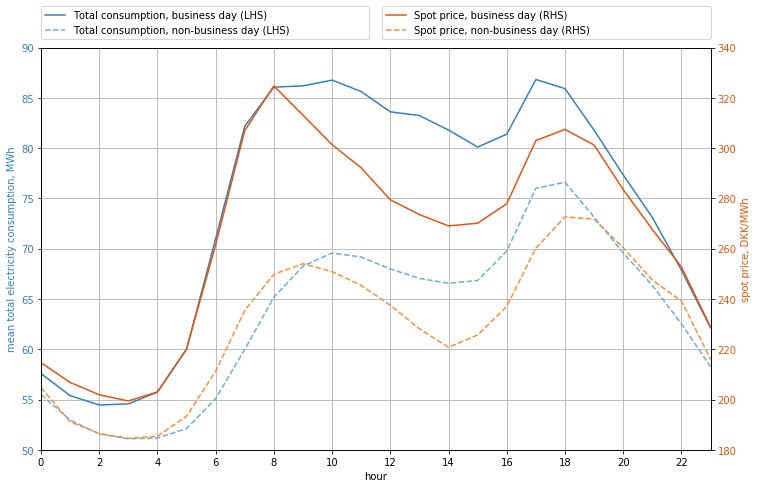
\includegraphics[width=1. \textwidth]{03_figures/hours}
  \label{fig:cons_hour}
\end{figure}


\subsection{Spot market prices and wind power prognosis}
\label{subsec:d_spot}
We include the hour-by-hour spot market price on the day-ahead-market for the price region DK1 or DK2 depending on where the grid company is located (see section \ref{subsec:t_market}).
\begin{figure}[H]
  \centering
  \caption{Time series for spot price and total consumption (business days)}
  \label{fig:price_cons_time_series}
\end{figure}
An important factor for the spot price on the day-ahead-market is the hour-by-hour wind power prognosis\footnote{'Elspot prices' and 'Wind power prognosis' by price region and year is updated daily after 2PM by Nord Pool and downloadable at \href{https://www.nordpoolgroup.com/historical-market-data/}{nordpoolgroup.com/historical-market-data}} for the following day.
\begin{figure}[H]
  \centering
  \caption{Wind power prognosis and spot price by hour (business days)}
  \label{fig:wp_price_hour}
\end{figure}

\begin{table}[H]
  \centering
  \caption{Correlation matrix for consumption, spot price, and wind power prognosis}
  \footnotesize
  \label{tab:correlation}
\end{table}


\subsection{Time-of-use tariff}
\label{subsec:d_tout}
From December 2017 grid companies have been allowed to introduce time-of-use (TOU) tariffs for retail consumption in order to send signals that can direct the more flexible tasks away from the peak hours around dinnertime. Thus, two of the bigger grid companies have already introduced TOU tariffs for the peak-hours 5-7 PM (from here written as hours 17-19) for the months October-March in which electricity consumption is also higher due to the lack of daylight. While NRGI initially only runs an experiment for a smaller group of flex-settled consumers Radius is introducing a full-scale TOU tariff scheme while exchanging the old prepayment meters with smart meters for the 600,000 retail customers in the Copenhagen metropolitan area.\footnote{See \href{https://ing.dk/artikel/nu-loebes-fleksible-elforbrug-omsider-gang-209251}{ing.dk/artikel/nu-loebes-fleksible-elforbrug-omsider-gang-209251} (Danish).}
\par
The variable for the TOU tariff represents the share of retail customers in Radius exposed to the tariff. As seen in Figure \ref{fig:cons_meters_time_series} and Table \ref{tab:descriptive} below the increasing share ends near 60 pct. in December 2018.
\begin{figure}[H]
  \centering
  \caption{Time series for retail consumption and no. meters in Radius}
  \label{fig:cons_meters_time_series}
\end{figure}

\subsection{Weather data}
\label{subsec:d_weather}
The outside temperature is relevant to the extent that electrical heaters or air conditioning is used \citep{lijesen2007real, vesterberg2014residential}. As the electricity consumption ceteris paribus is expected to be higher for both low-end and high-end temperatures, $temperature^2$ is included as well.\footnote{Scraped via iterative lookups in the records of the Danish Meteorological Institute at \href{https://www.dmi.dk/vejrarkiv/}{dmi.dk/vejrarkiv/}}
\medskip\\
Lighting is used more in the absence of daylight. Therefore, an indicator for daytime is included such that $daytime=1$ for hours between sunrise and sunset and e.g. $daytime=0.25$ for $hour=7$ if sunrise was a quarter past 7.\footnote{Sunrise and sunset are scraped for each date in the sample via iterative lookups at \href{https://soltider.dk/}{soltider.dk}}
\medskip\\
Taking advantage of the dense size of Denmark, temperature and daytime are not scraped by the location of each of the 52 grid companies which often cross municipality-borders but for the two most populace municipalities and applied to all grids within that price region.\footnote{Temperature is for the municipalities of Aarhus and Copenhagen respectively while sunrise and sunset are for the City Hall Square in each of the two cites.}

\subsection{Time variables}
\label{subsec:d_time}
Year dummies as well as a time trend indicating the number of days since January 1 2016 are included to account for economic growth (increase), technological progress (decrease) \citep{lijesen2007real}, or compositional changes that can affect electricity consumption other than the number of meters.
\medskip\\
Danish bank holidays as well as a few other common holidays with lower wholesale electricity consumption\footnote{January 2 (the day after New Year's Day), May 1 (International Workers' Day), Friday after Ascension Day, June 5 (Constitution Day), last Friday before Christmas, and the days between Christmas and New Year's. All holidays according to \href{https://kalendersiden.dk/}{kalendersiden.dk}} are taken into account in order to do sample split regressions for business days and non-business days, the latter including holidays and weekends.
\begin{verbatim}
   \begin{table}[H]
  \centering
  \caption{Descriptive statistics}
  \footnotesize
    \begin{tabular}{l*{1}{ccccc}}
\hline\hline
                    &\multicolumn{5}{c}{}                                            \\
                    &        mean&          sd&         min&         p50&         max\\
\midrule
Wholesale electricity consumption, MWh&    34.17217&     83.3248&     .063157&      5.9281&    757.5571\\
Retail electricity consumption, MWh&    28.74596&    74.08786&           0&    5.833275&    906.3964\\
Number of wholesale meters&    923.9638&    2440.423&           7&       140.5&       17674\\
Number of retail meters&    57551.23&      148260&         858&       14371&     1006061\\
- of which flex-settled&    4299.473&    37193.14&           0&           0&      596267\\
- of which residual &    53251.75&    134556.1&         855&       14357&      998864\\
Electricity spot price, DKK&    252.9863&    108.0154&     -398.61&      234.94&      1898.9\\
Wind power prognosis for DK1, GWh&    1.225359&    .9221094&           0&       1.002&       3.973\\
Wind power prognosis for DK2, GWh&    .3266759&    .2702798&           0&        .249&       1.084\\
wp                  &    1.075578&    .9126432&           0&        .796&       3.973\\
wp\_other            &    .4764563&    .5610359&           0&         .31&       3.973\\
Wind power prognosis for Sweden, GWh&    1.862874&    1.118507&        .062&       1.668&        5.84\\
Price region DK1 (Western Denmark)&    .8333333&    .3726781&           0&           1&           1\\
Share time-of-use tariff&    .0001378&    .0079703&           0&           0&    .5926748\\
Temperature         &    9.094615&    6.915881&       -11.9&         8.7&        31.4\\
Daytime             &    .5135309&    .4857462&           0&    .6666667&           1\\
Time trend          &    547.4559&    316.4119&           0&         547&        1095\\
Holiday (not in a weekend)&    .0437643&    .2045702&           0&           0&           1\\
\midrule
Observations        &     1420200&            &            &            &            \\
\bottomrule\end{tabular}

  \label{tab:descriptive}
\end{table}  
\end{verbatim}

